\chapter{Testüberdeckung}

Um die Testüberdeckung zu maximieren, wurden noch mehrere automatische Unittests geschrieben. In diesem Kapitel finden sie kurze Beschreibungen zu den verwendeten Testverfahren und das Endergebnis der Testüberdeckung.
\section{Unittests}
\subsection{Tests des Cron Moduls}
Im Cron Modul wurden die Methoden getestet, die in bestimmten Zeitabschnitten regelmäßig ausgeführt werden sollen. Es wurde getestet, ob die Änderungen zwischen den ersten Aufruf einer Methode und der nachfolgenden zu dem gewünschten Ergebnis führen. Da die Mehrheit der Methoden aus dem Cron Modul ständig einen WPS Server für die Kommunikation brauchen, ist es kompliziert die Testüberdeckung zu maximieren.
\subsection{Tests des View Moduls}

Das Format vom Datenaustausch zwischen Client und Server ist fest spezifiziert. Dazu gehört der Standard (\gls{JSON}), sowie auch Attributnamen und Verschachtelung der Objekte (z.B. ein Workflow enthält mehrere Tasks, und jeder Task enthält wiederum mehrere Artefacts). Die Aufgabe der Unit-Tests für die Views ist es, sicherzustellen, dass, wenn der Server eine Anfrage mit Daten im korrektem Format bekommt, dieser sich auch richtig verhält. Die aktuelle Testüberdeckung in diesem Teil des Servers beträgt ca. 90\%.

\subsection{Tests des Utils Moduls}
Es wurden mehrere Test wurden, um die korrekte Ausführung der Funktionen in der utils.py Datei sicherzustellen. Besonderen Wert wurde auf die Funktionen gelegt, die sich mit dem \gls{Parsen} von XML Dateien beschäftigen, da die Funktionalität für die Kommunikation mit dem WPS Server essentiell ist. Dafür wurden statische XML Dateien angelegt, die den Responses von WPS Servern entsprechen. \newline
Dazu gehören auch zahlreiche Tests, die die Reaktion der Datenbank auf verschiedene Ereignisse überprüfen. Zum Beispiel, dass nach dem Hinzufügen eines WPS Prozesses der bereits in der Datenbank existiert kein neuer Datensatz erzeugt wird, sondern der alte aktualisiert wird.


\newpage
\section{Ergebnis}

Der aktuelle Stand der Testüberdeckung ist 80\%

\begin{figure}[H]
    \centering
    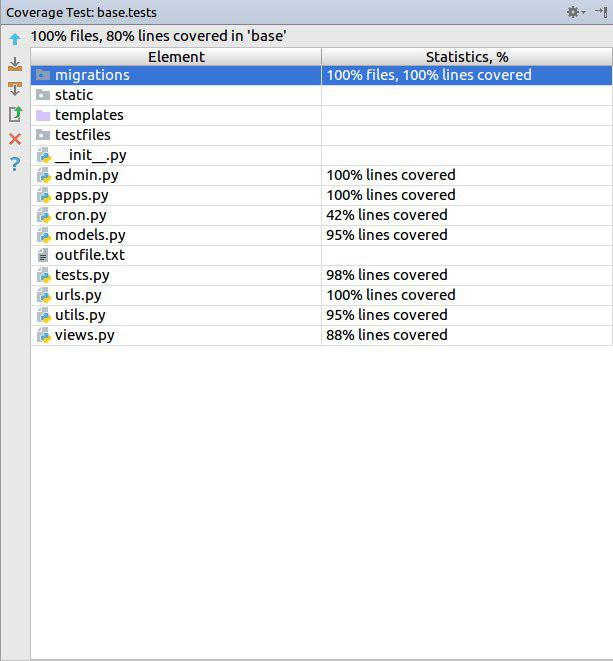
\includegraphics[width=15cm]{images/Coverage_white.jpg}
    \caption{Testüberdeckung der Endversion}
    \label{Ergebnis2}
\end{figure}
